%\chapter{\ecal simualtion study for upgradeII}

\section{Parameterized simulation}


The parameterized simulation tool is developed to study the requirements to \ecal for \upgradetwo with pretty high instananeus lominosity.
This tool is based on \gauss\supercite{LHCb-PROC-2011-006} and \delphes\supercite{delphes_paper},
\gauss\supercite is used to produce generated level sample with different eventtypes
\footnote{Different eventtypes present different decay channels.} 
and \delphes is used to run detector simulation by parameterized way.
Actually,
the \delphes does not have appropriate module easyly used for \ecal simulation for \lhcb, 
since the default geometry of calorimeter in \delphes is bucket,
while the geometry of \ecal at \lhcb  is a plane.
Therefore,
new parameterized simulation modules for \lhcb is developed first. 
Then, 
the specific decay channels are reconstructed using the output from parameterized simulation.
Finally,
these simulation samples are analyzed.
The frame to achieve the parameterized simulation for \ecal is shown in Figure.~\ref{fig:process_fast}

%%%%%%%%%%%%%%%%%%%%%%%%%%%%%%%%%%%%%%%%
\begin{figure}[!htb]
  \begin{center}
    \includegraphics[width=0.95\linewidth]{Figures/06_ECAL/fast_sim/process_fast}%\put(-32,133){(a)}
    \vspace*{-0.5cm}
  \end{center}
  \caption{
   The simulation process in the parameterized simulation.
  }
  \label{fig:process_fast}
\end{figure}
%%%%%%%%%%%%%%%%%%%%%%%%%%%%%%%%%%%%%%%%



\subsection{Parameterization of shower}

A method to achieve parameterized simualtion is introduced below briefly.
The particles like photon or electron will transform into electromagnetic showers in \ecal,
which are consisted of many electrons or photons.
Two processes, photon pair production and electron bremsstrahlung, 
continue with the shower development until photons fall below the pair production threshold.
Then mean longitudinal profile of the energy deposition in electromagnetic cascade can be discribed by this formula obtained from beam test\supercite{Levy:2017lpw}:
\begin{equation}
F(x,y,f,\sigma,R) = \frac{f}{2\pi\sigma}e^{-\frac{x^2+y^2}{2\sigma^{2}}} + \frac{1-f}{2\pi}\frac{2R^2}{(x^2+y^2+z^2)^2}
\end{equation}
where the first part is used to discribe the tail of shower,
and the second part to discribe the main section.
The parameters used can obtained from the beam test, like $\sigma$, $f$ and $R$.
Above formular is utilized to distribute the energy of entering particle to the corresponding cells.
In the parameterized simulation tool,
the length of the cascade shape is not considered.

Next step is to smear the deposited energy in the cell, 
the parameterized energy resolution formula is used:
\begin{equation}
\frac{\sigma}{E} = \frac{\alpha}{\sqrt{E}} \oplus \beta
\end{equation}
where $\alpha$ is roughly equal to 10\% and $\beta$ is approximately equal to 1\% for the current shashlik \ecal, 
as mensioned in Section.~\ref{subsubsec:calorimter}.
After \upgradetwo at \lhcb,
the measuring unit of \ecal will have have ability to record precision time information,
the time resolution is a given value in this simulation tool,
it is convenient to set this value in the configuration file.


\subsection{Reconstuction and calibration}

The reconstruction method in the parameterized simualtion tool follows the one utilized in the current shashlik \ecal,
which is named as cellular automaton algorithm\supercite{Breton:2001tua,Deschamps:691634}.
This method is processed based on the seed cell, 
which has a local maximum energy.
In this tool,
the clusters are determined by the algorithm mentioned above,
and reconstructed unsing $3\times3$ cells,
the energy and position are calculated as:
\begin{equation}
\label{eq:rec}
\begin{split}
   E = \sum_{i}^{cells}{E_i} \\
   x_{c} = (\sum_{i}^{cells}{x_i \times E_i})/E \\
   y_{c} = (\sum_{i}^{cells}{y_i \times E_i})/E \\
   z_{c} = z_i \\
   t_{c} = (\sum_{i}^{cells}{t_i \times E_i})/E
\end{split}
\end{equation}
where the subscript $i$ represents the cell belonging to the corresponding cluster.

\begin{figure}[!thbp]
\centering
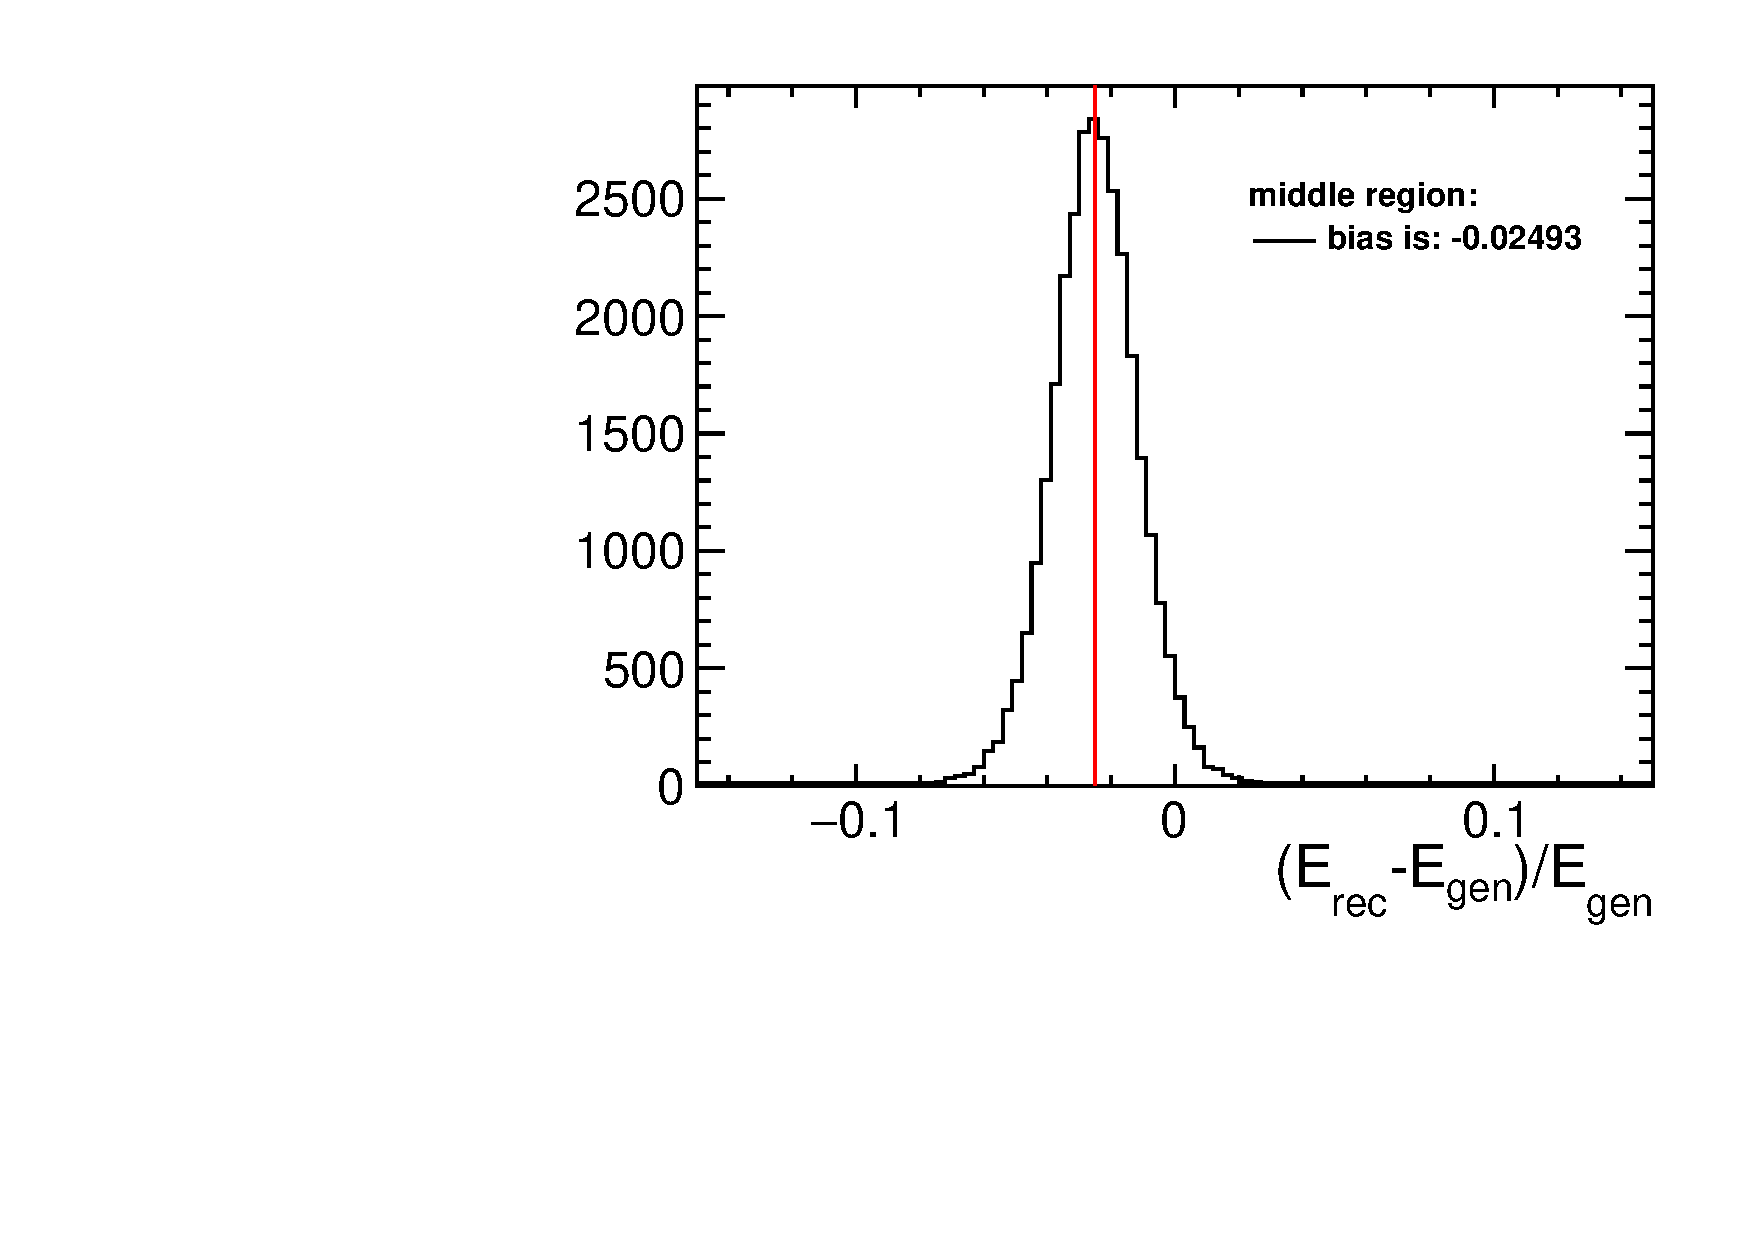
\includegraphics[width=0.43\textwidth]{Figures/06_ECAL/fast_sim/for_fast_cali/energy_cali/energy_cali/middle_energy.pdf}
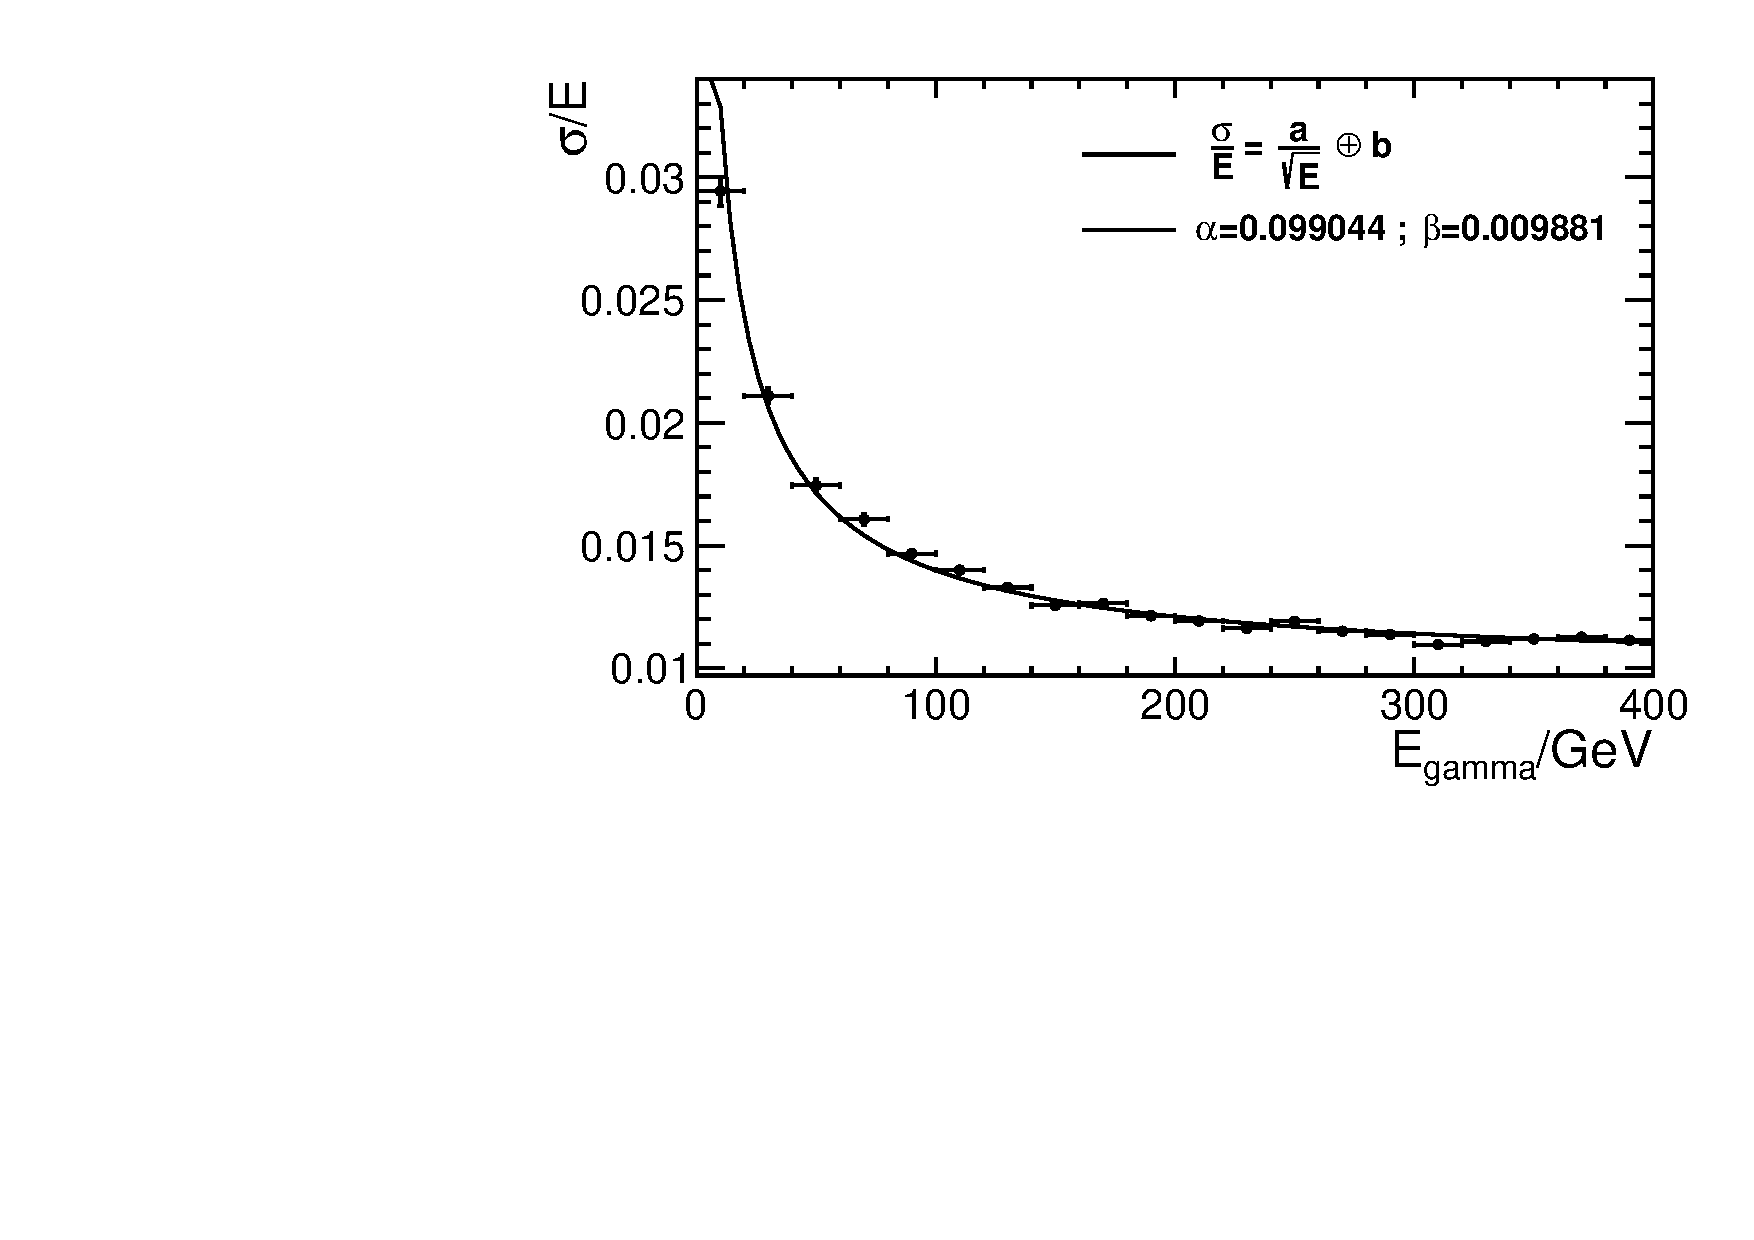
\includegraphics[width=0.49\textwidth]{Figures/06_ECAL/fast_sim/for_fast_cali/energy_cali/res_ene.pdf}
   \caption{The difference between the reconstructed energy and generated level energy  (left),
   and the relation between the energy resolution and particle energy after calibration (right).}
\label{fig:fast_ene_cali}
\end{figure}

In this tool,
the calibration to the reconstructed variables are also imported.
The energy need to be recaculated by multiplying with a factor due the energy leaking effect.
The bias between the reconstructed energy and generated energy is shown in left of Figure.~\ref{fig:ene_cali}.
In addition,
the calibration to the position is achieved by using a correction formula:
\begin{equation}
\label{eq:pos_cali}
x_{cali} = f \times b \times asinh(\frac{x_{rec}}{\Delta}cosh\frac{\Delta}{b})
\end{equation}
where the $x_{cali}$ is the x-coordinate in the frame of seed cell,
$x_{rec}$ the position obtained from Equation.~\ref{eq:rec},
and other variables are calibration parameters.
The performance of position calibration is shown in the Figure.~\ref{fig:pos_cali},
which is in the case of cell size equal to $6.06\cm$.
By the way,
the calibration need to be applied indepently to the sample using different cell size.

To verify the credibility of this method, 
the energy resolution is checked by \g gun events,
as shown in the right of Figure.~\ref{fig:fast_ene_cali},
which is consistent to the performance of current \ecal.

\begin{figure}[!thbp]
\centering
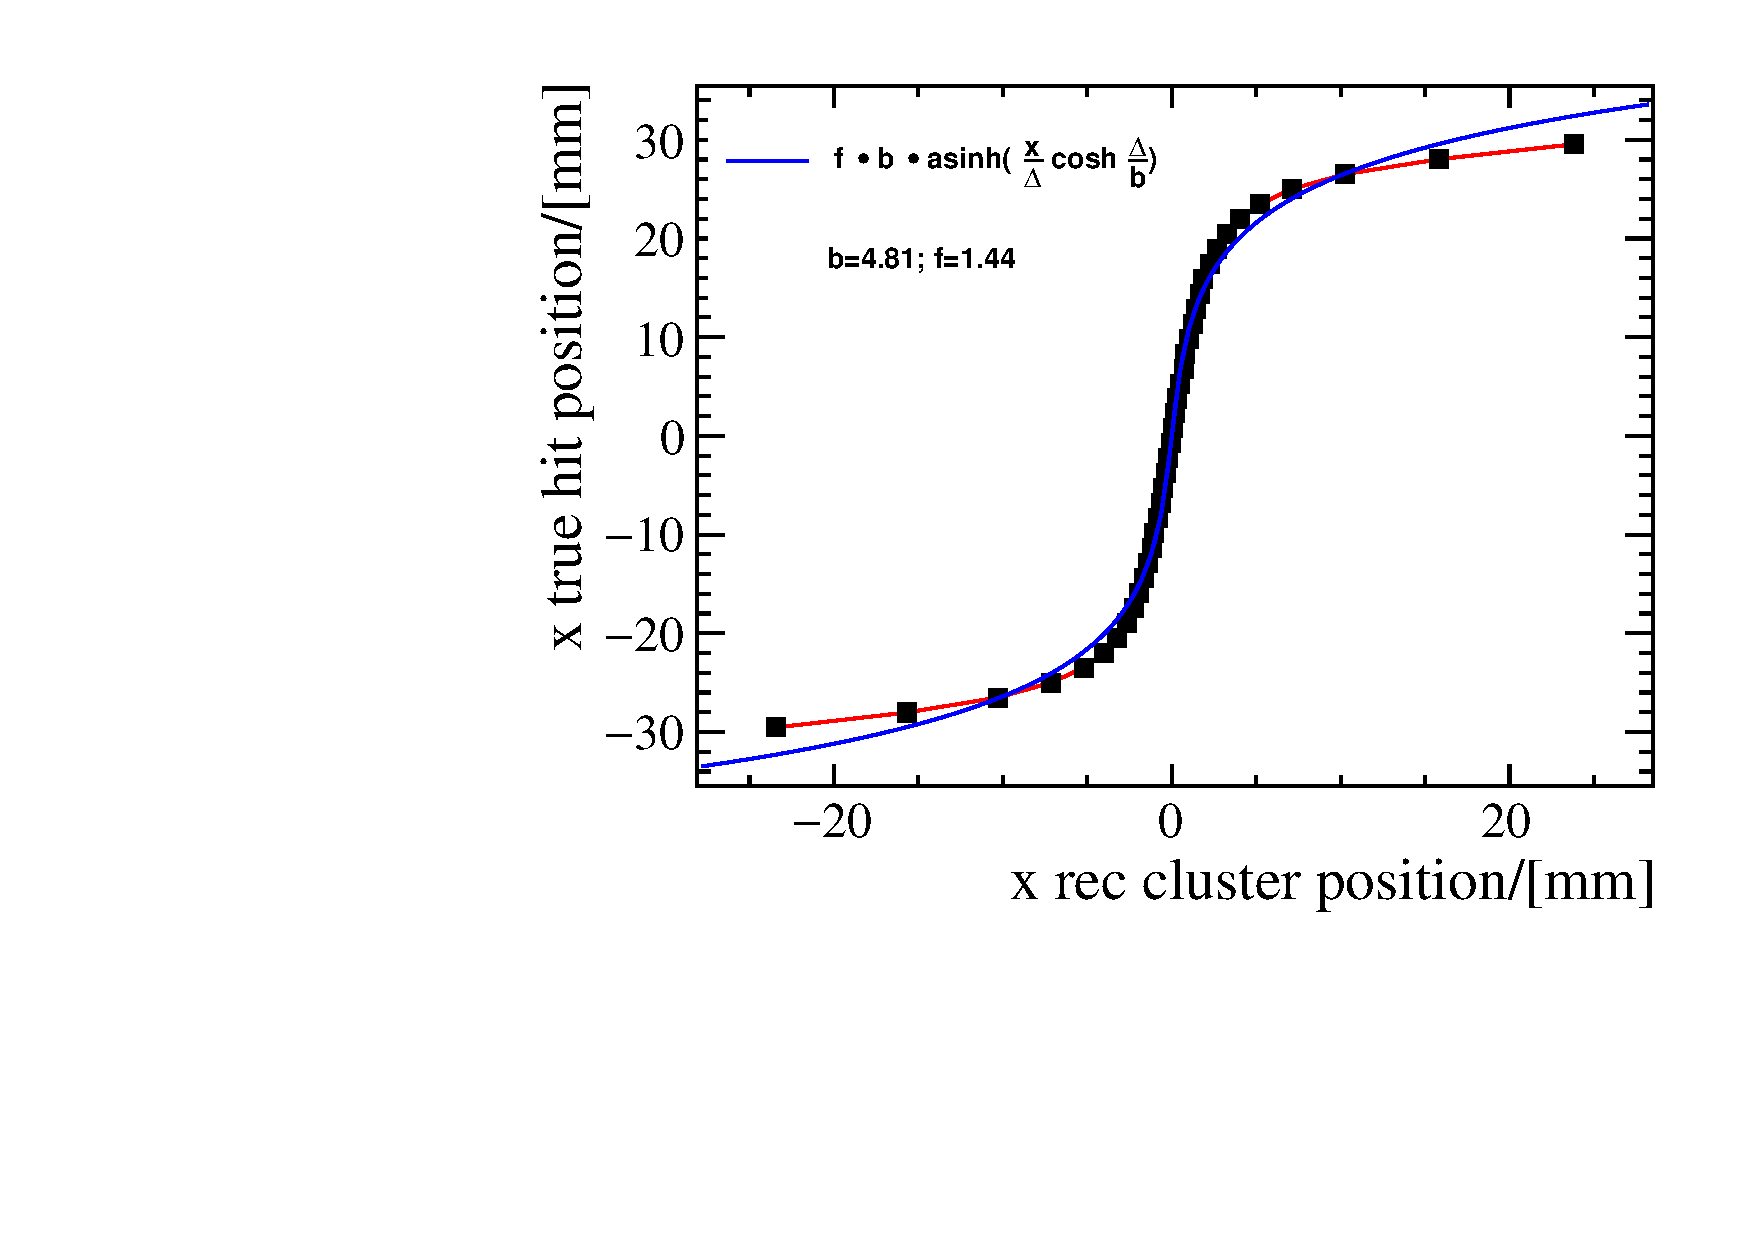
\includegraphics[width=0.49\textwidth]{Figures/06_ECAL/fast_sim/for_fast_cali/S_correction/before/middle_cor.pdf}
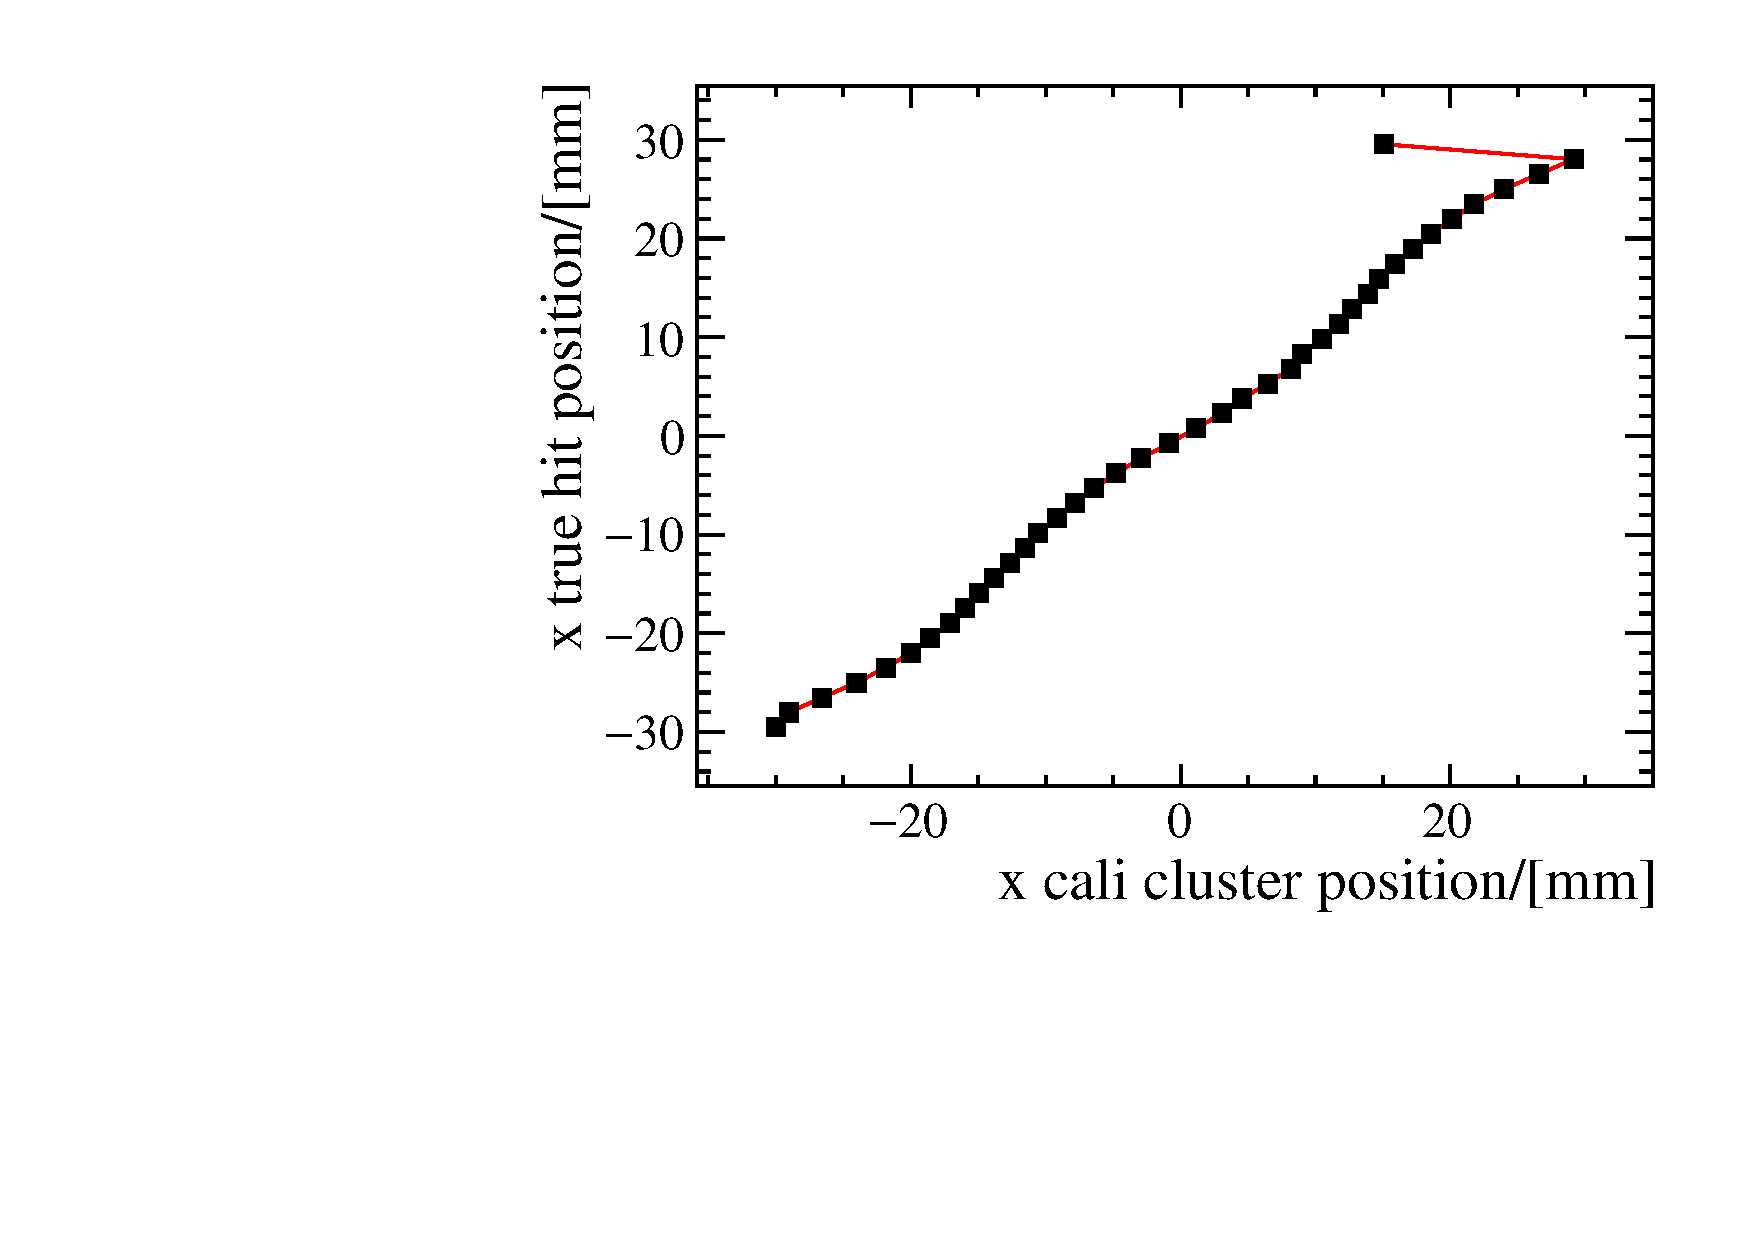
\includegraphics[width=0.49\textwidth]{Figures/06_ECAL/fast_sim/for_fast_cali/S_correction/after/middle_cor.pdf}
   \caption{The relation between the true position and reconstructed position before (left) and after (right) calibration.}
\label{fig:fast_pos_cali}
\end{figure}



\subsection{Neutral particle identification}
\label{subsec:ecal_identification}

\subsubsection{Removal of charged particles}
Some charged particles can also deposit energy in \ecal, 
we can removed this effect by an anti-coincidence between the cluster ($\et>250\mev$) position 
and the extrapolation of the reconstructed tracks ($\pt>150\mev$) up to the calorimeter.
The distance between the reconstructed cluster and the nearest tracks is calculated,
if the position resolution of tracks is overlooked, 
the required distrance is larged than half of the cell size. 
If the futher trackers and \ecal both have ability to record precision time,
the time matching between track arrival time and shower reconstructed time can also help to identify the cluster arised from charged particle.


\subsubsection{Characteristics of $\gamma, \piz$ and overlapping cluster}

$\gamma\slash\piz$ seperation is an important prerequisite for many physics analysis\supercite{CalvoGomez:2042173}.
Many photons detected by the \ecal are originated from \piz decays.
Two photons of the \piz has possibility to be reconstructed as one cluster due to the granualarity,
especially for the \piz with pretty large momentum,
as shown in the Figure.~\ref{fig:pi0_distance_E}.
If the distance between 2$\gamma$ decayed from the $\piz$ in the \ecal plane is large enough,
the \piz can be reconstructed as resolved one,
otherwise,
it will be reconstructed as merged particle,
which means the showers from the 2$\gamma$ are overlapping together.



%The reconstruction performance of \piz will reflect the separation ability of this \ecal.
%The distance of two $\gamma$ onto the \ecal plane is related to the \piz energy, as shown in the Fig.~\ref{fig:pi0_distance_E}.

%From the left plot,
%we find almost all \piz with energy smaller than 150\gev can be reconstructed as resolved \piz,
%as the distance between the decaying two $\gamma$ on the \ecal plane is larger than $30\mm$.
%Actually,
%the \piz energy in some decay channels studied at \lhcb is smaller than 100\gev,
%such as $\Bs\to\jpsi\piz$,
%some specific physical channels performance with this high granularity \ecal will be discussed later.

\begin{figure}[!htbp]
\centering
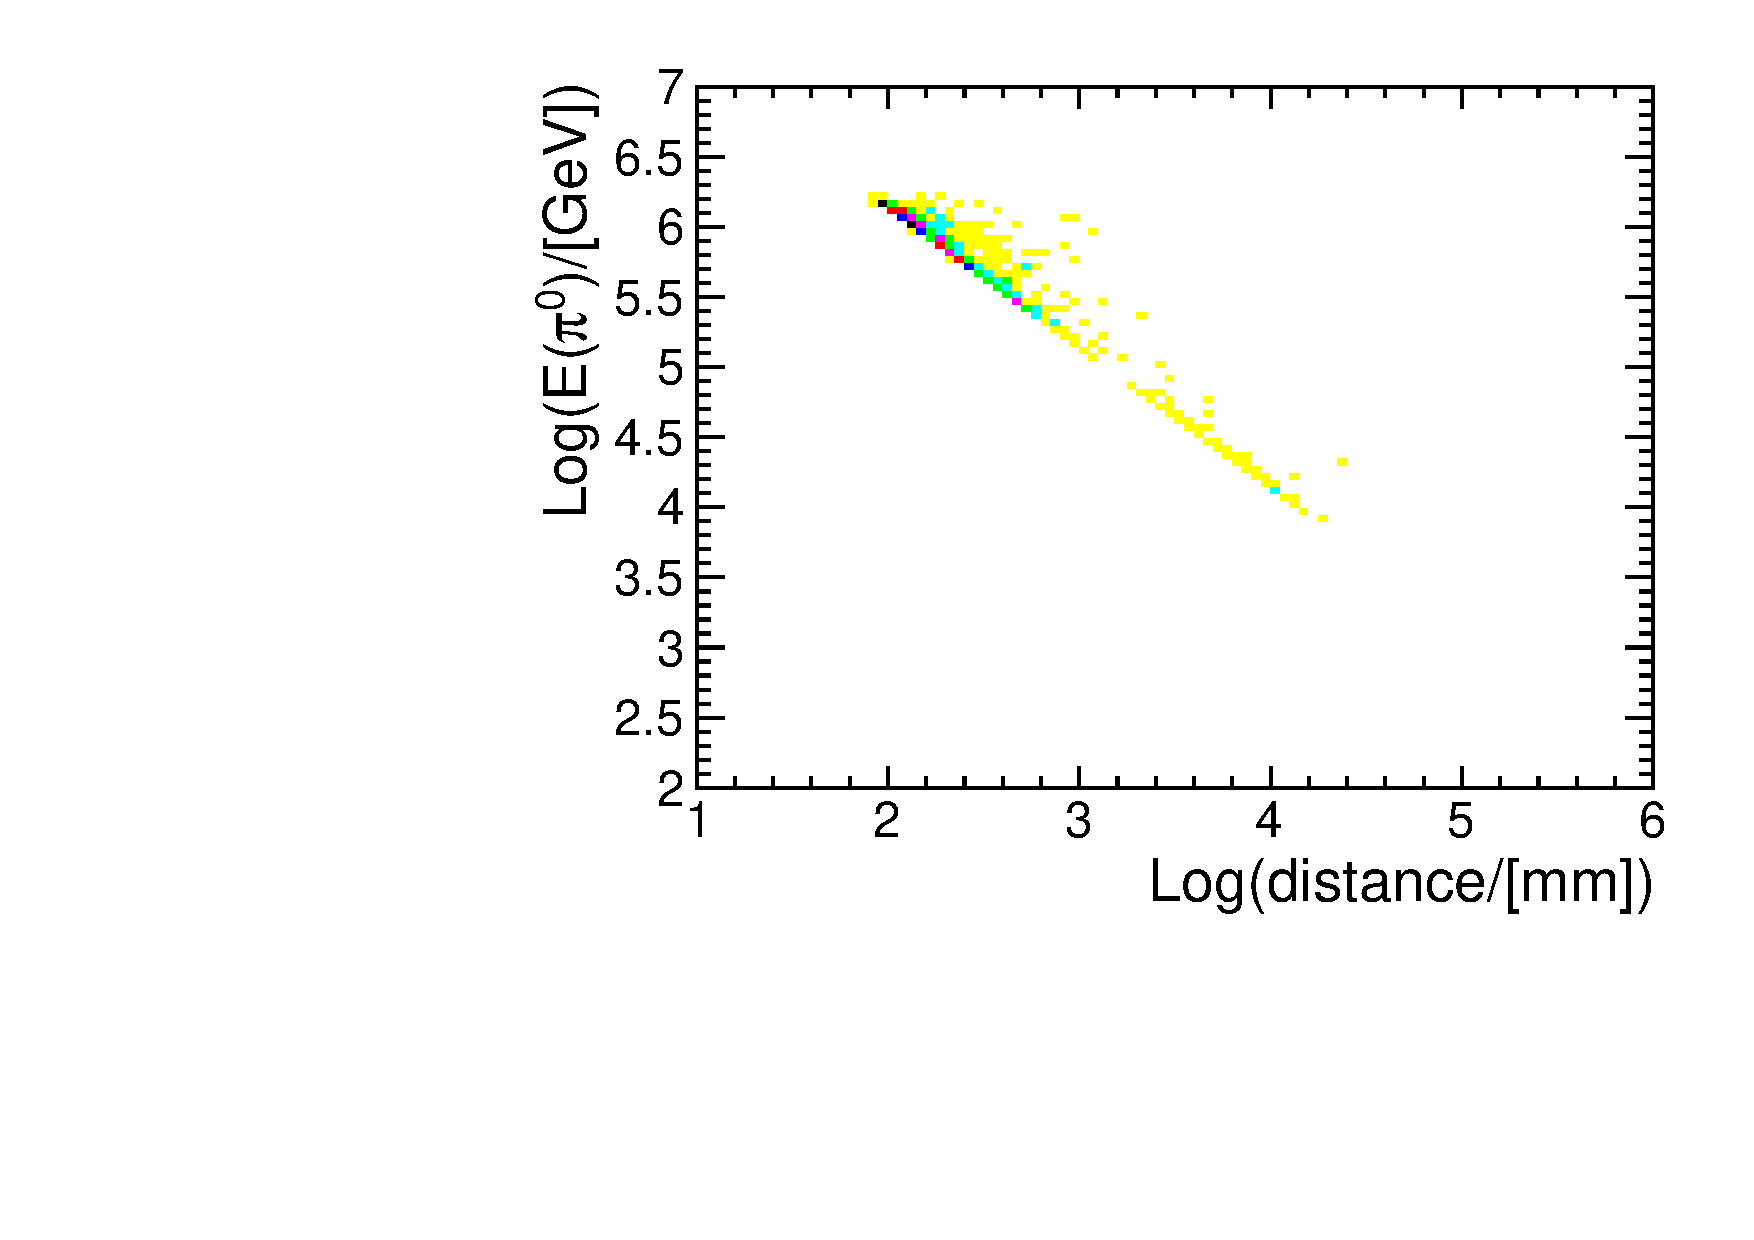
\includegraphics[width=0.45\textwidth]{Figures/06_ECAL/pi0_plots/distance_E.pdf}
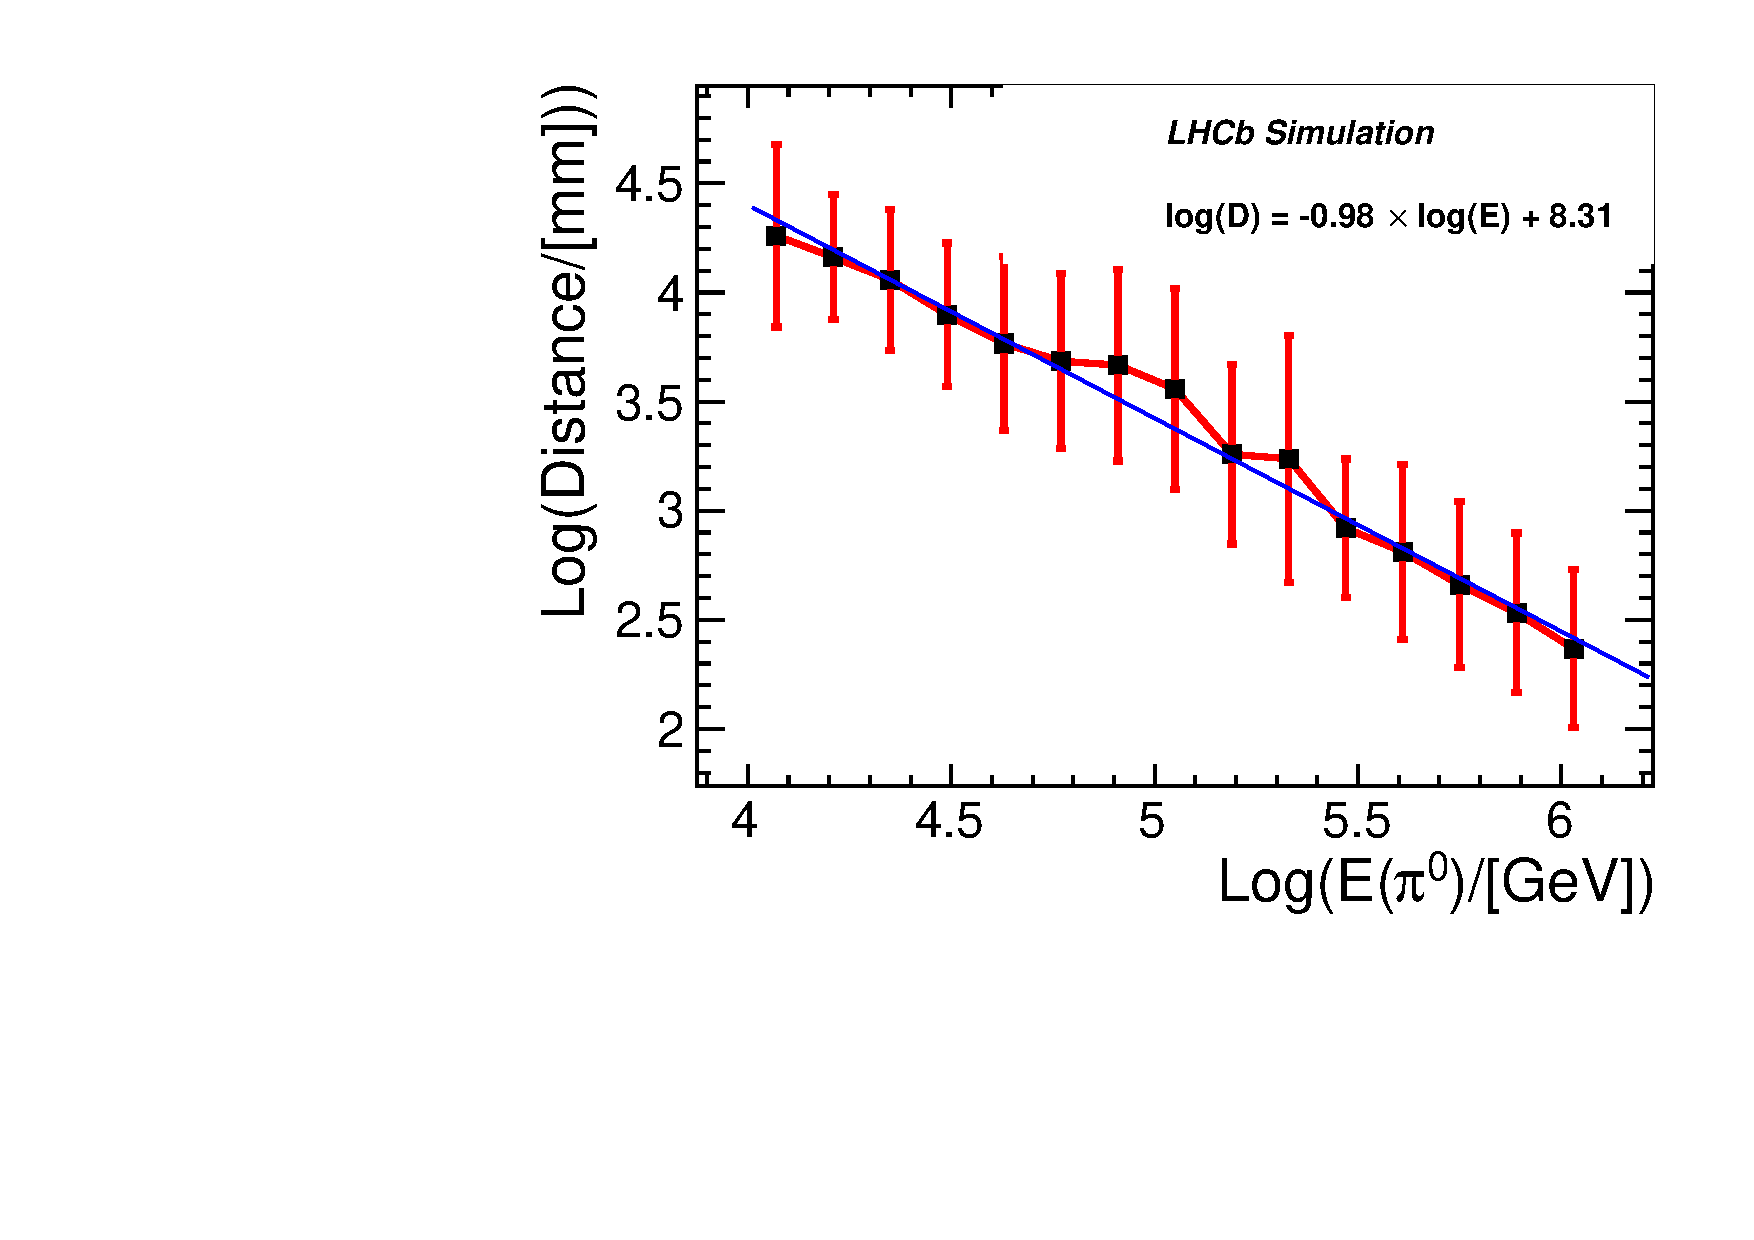
\includegraphics[width=0.45\textwidth]{Figures/06_ECAL/pi0_plots/distance_E_1D.pdf}
\caption{The relation between the \piz energy and the distance of two $\gamma$ on the \ecal plane.} 
\label{fig:pi0_distance_E}
\end{figure}

As the luminosity will become pretty high after \upgradetwo, 
it is possible to increase the chances of overlapping clusters.
%Using the cell with small size and small Moli\`ere radius is a possible method to reduce this kinds of bankground candidates,
%this will be dicussed in Section.~\ref{}.
And beyond that,
Identifying the random overlapping cluster is another important task.


The method for $\gamma, \piz$ and overlapping cluster seperation is based on the shape of cluster.
As the timing information will be recorded after \upgradetwo, 
it also has possibility to seperate the clusters from different sources.
The position spread matrix elements are defined as:
\begin{equation}
\label{eq:spread_matrix}
\begin{split}
   S_{XX} = \frac{\sum_{i=1}^{N}E_{i}(x_{i}-x_{c})^2}{\sum_{i=1}^{N}E_{i}} \\
   S_{YY} = \frac{\sum_{i=1}^{N}E_{i}(y_{i}-y_{c})^2}{\sum_{i=1}^{N}E_{i}} \\
   S_{XY} = \frac{\sum_{i=1}^{N}E_{i}(x_{i}-x_{c})(y_{i}-y_{c})}{\sum_{i=1}^{N}E_{i}} \\
\end{split}
\end{equation}
where $(x_c,y_c)$ is the position of the cluster, as defined in Equation~\ref{eq:rec},
and $(x_i,y_i)$ is the position of used cell for a given cluster of $N$ cells.
In this simualtion, 
seven separation variables are constructed including timing information:
\begin{itemize}

\item The size of the cluster, also explained as second order of moments, refered to as $r2$:
\begin{equation}
   r2 = <r^2> = S_{XX} + S_{YY}
\end{equation}

\item The importance of the tails, refered to as $r2r4$:
\begin{equation}
   r2r4 = 1- \frac{ <r^2>^2 }{ <r^4> }
\end{equation}

\item Ratio of the eigenvalues of the matrix $S$:   
\begin{equation}
   \kappa = \sqrt{ 1-4\frac{S_{XX}S_{YY}-S^2_{XY}} {(S_{XX}+S_{YY})^2} } 
\end{equation}

\item The orientation of the correlation between $X$ and $Y$ coordinates, refered to as $asym$:
\begin{equation}
   asym = \frac{S_{XY}}{\sqrt{S_{XX}S_{YY}}}
\end{equation}

\item The energy fraction of the seed cell in the cluster:
\begin{equation}
   E_{seed} \slash E_{cluster}
\end{equation}

\item The second order of moments about timing information, refered to as $r2$:
\begin{equation}
   t2 = <t^2> = \frac{\sum_{i=1}^{N}E_{i}(t_{i}-t_{c})^2}{\sum_{i=1}^{N}E_{i}} 
\end{equation}

\item The importance of the tails of timing, refered to as $t2t4$:
\begin{equation}
   t2t4 = 1- \frac{ <t^2>^2 }{ <t^4> } 
\end{equation}

\end{itemize}

The variables constructed above are taken as input for the multi-varible analysis tool,
several methods are compared, 
and the BDTG is taken as the default trainning algorithm.


\subsubsection{$\gamma, \piz$ and overlapping cluster separation}

The discriminant variables introduced above are taken as input for Multivariate Analysis (TMVA)\supercite{TMVA4}.
Photons in \lhcb acceptance with $E\in[10,400] \gev$ events are taken as signal sample (EventType=56000400). 
The \piz particle gun decaying to two \g events are generated used for the merged \piz smaple (EventType==56200100).
Furthermore, 
the random overlapping cluster sample is created base on the gamma gun events, 
with a gamma particle is inserted in the generated level.
The energy of accompaning gamma with the exponential distribution, 
with the mean value equl to $10 \gev$,
which is estimated from the minimum bias sample.
The generated position and time of this accompaning gamma follow the charecter of primary vertex distribution.
Besides, 
$\et>250\mev$ is applied to all \g candidates before being imported in the TMVA tool.
Considering the energy scale of \g and \piz is defferent, 
$E<200 \gev$ is also applied to \g and random overlapping samples.  


Discrimination between \g and merged \piz is studied first.
Figure.~\ref{fig:identi_gamma_piz_var} shows these discriminant varibles used in the multivariable analysis,
while Figure.~\ref{fig:identi_gamma_piz_overtrain} shows the distribution of BDTG, 
and no overtaining effect appears from this test.
The receiver operating characteristic curve (ROC) is shown in Figure.~\ref{fig:identi_gamma_piz_ROC},
the left one is obtained with 8 discriminant variables are included, 
while the one shows the performance with only 6 variables (no $t2$ and $t2t4$ ).
According to these plots,
the timing information does not contribute much on the \g and merged \piz seperation.

%%%%%%%%%%%%%%%%%%%%%%%%%%%%%%%%%%%%%%%%
\begin{figure}[!htb]
  \begin{center}
    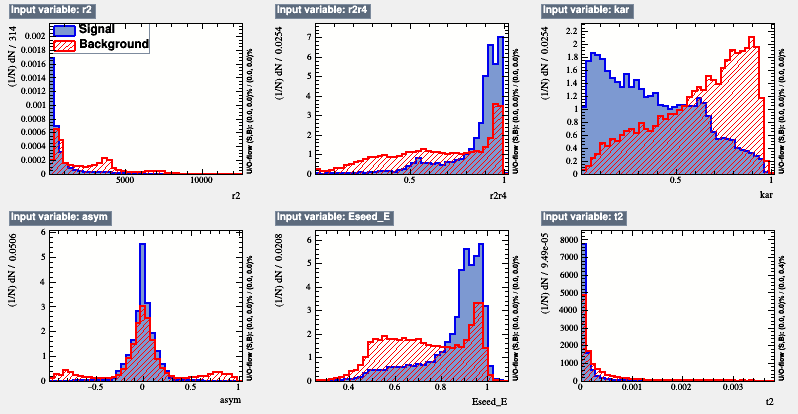
\includegraphics[width=0.99\linewidth]{Figures/06_ECAL/fast_sim/Identification/gamma_piz/with_time/variables_id_c1.png} \\
    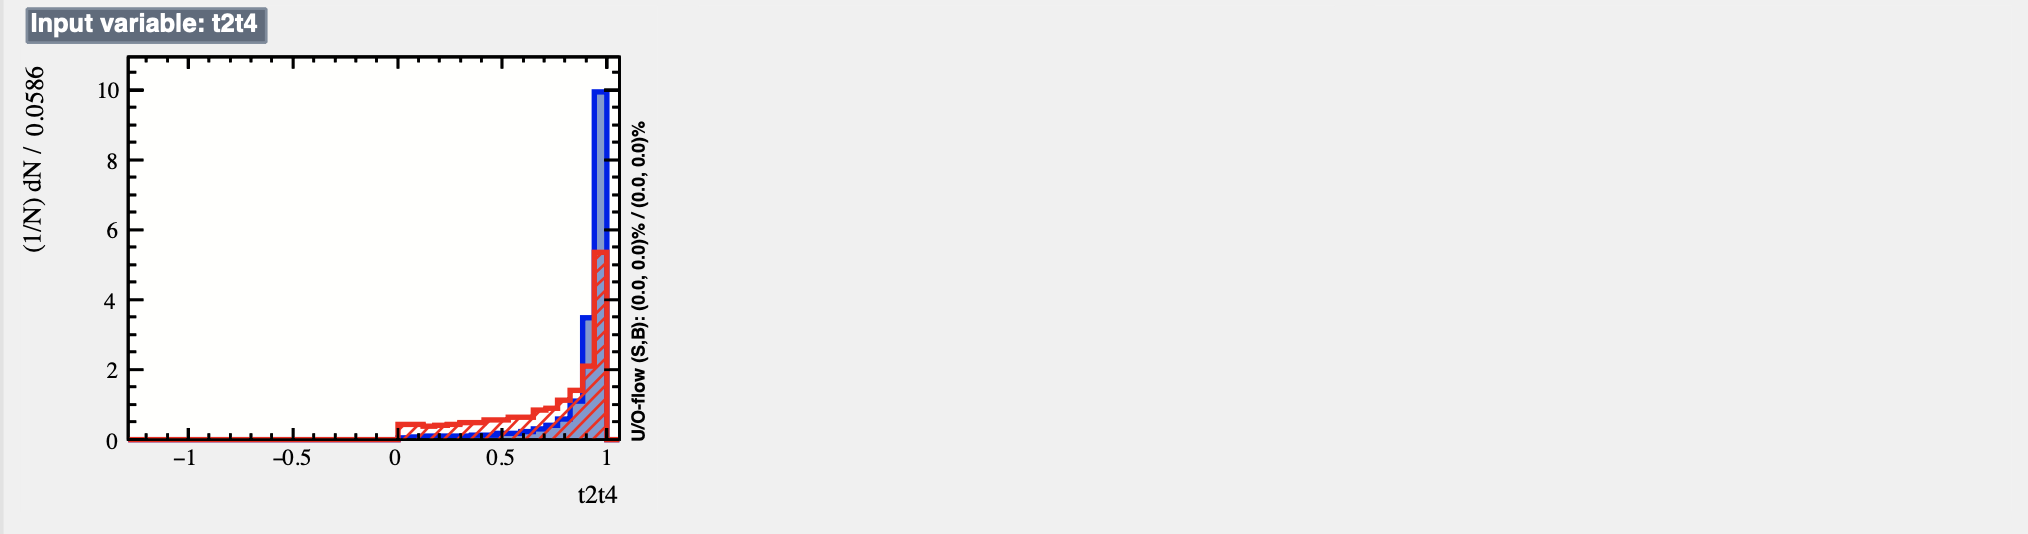
\includegraphics[width=0.97\linewidth]{Figures/06_ECAL/fast_sim/Identification/gamma_piz/with_time/new_variables_id_c2.png}
    \vspace*{-0.5cm}
  \end{center}
  \caption{
   The distribition of discriminant varibles used for cluster identification.
  }
  \label{fig:identi_gamma_piz_var}
\end{figure}
%%%%%%%%%%%%%%%%%%%%%%%%%%%%%%%%%%%%%%%%

%%%%%%%%%%%%%%%%%%%%%%%%%%%%%%%%%%%%%%%%
\begin{figure}[!htb]
  \begin{center}
    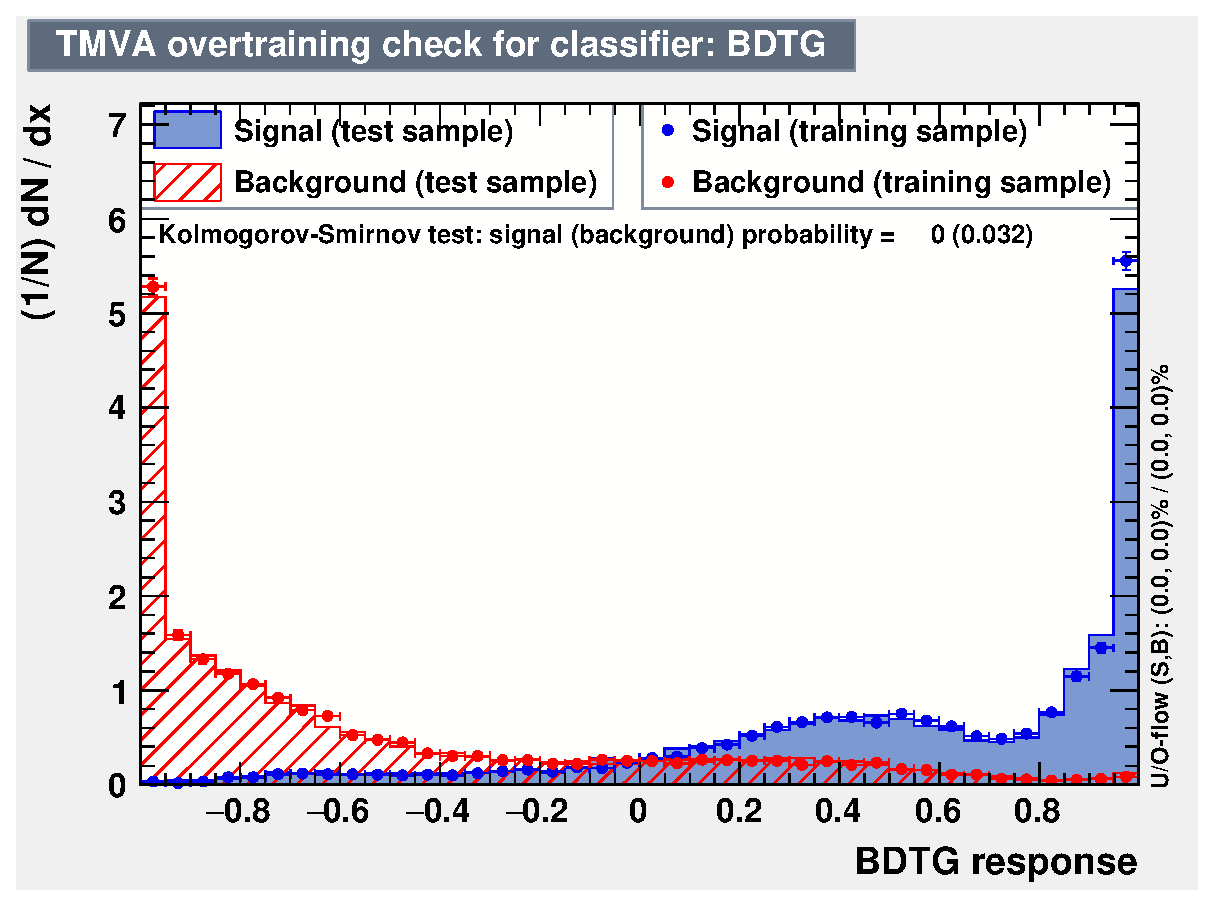
\includegraphics[width=0.49\linewidth]{Figures/06_ECAL/fast_sim/Identification/gamma_piz/with_time/overtrain_BDTG.eps} 
    \vspace*{-0.5cm}
  \end{center}
  \caption{
     The distribution of BDTG of the signal sample (\g) and background sample (merged \piz).
  }
  \label{fig:identi_gamma_piz_overtrain}
\end{figure}
%%%%%%%%%%%%%%%%%%%%%%%%%%%%%%%%%%%%%%%%

%%%%%%%%%%%%%%%%%%%%%%%%%%%%%%%%%%%%%%%%
\begin{figure}[!htb]
  \begin{center}
    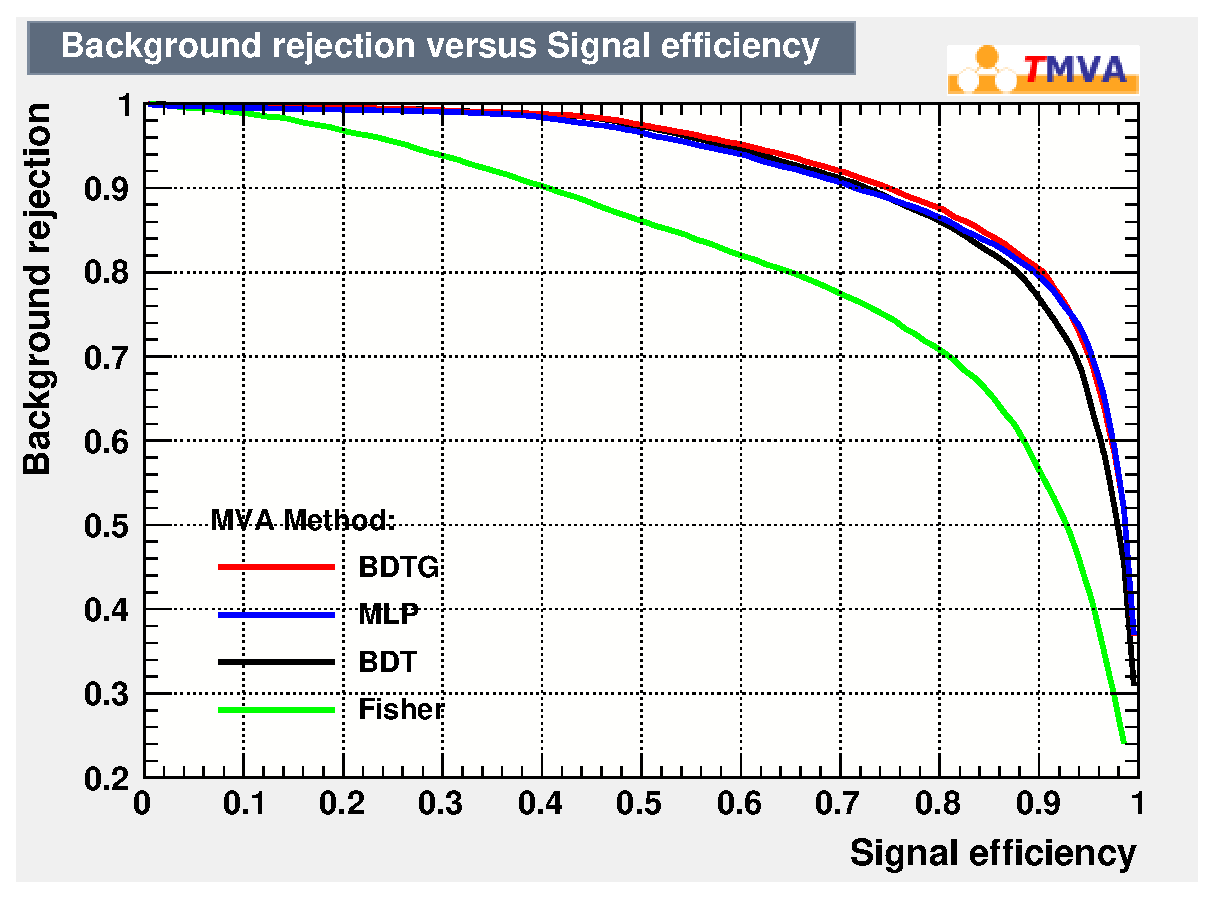
\includegraphics[width=0.49\linewidth]{Figures/06_ECAL/fast_sim/Identification/gamma_piz/with_time/rejBvsS.eps} 
    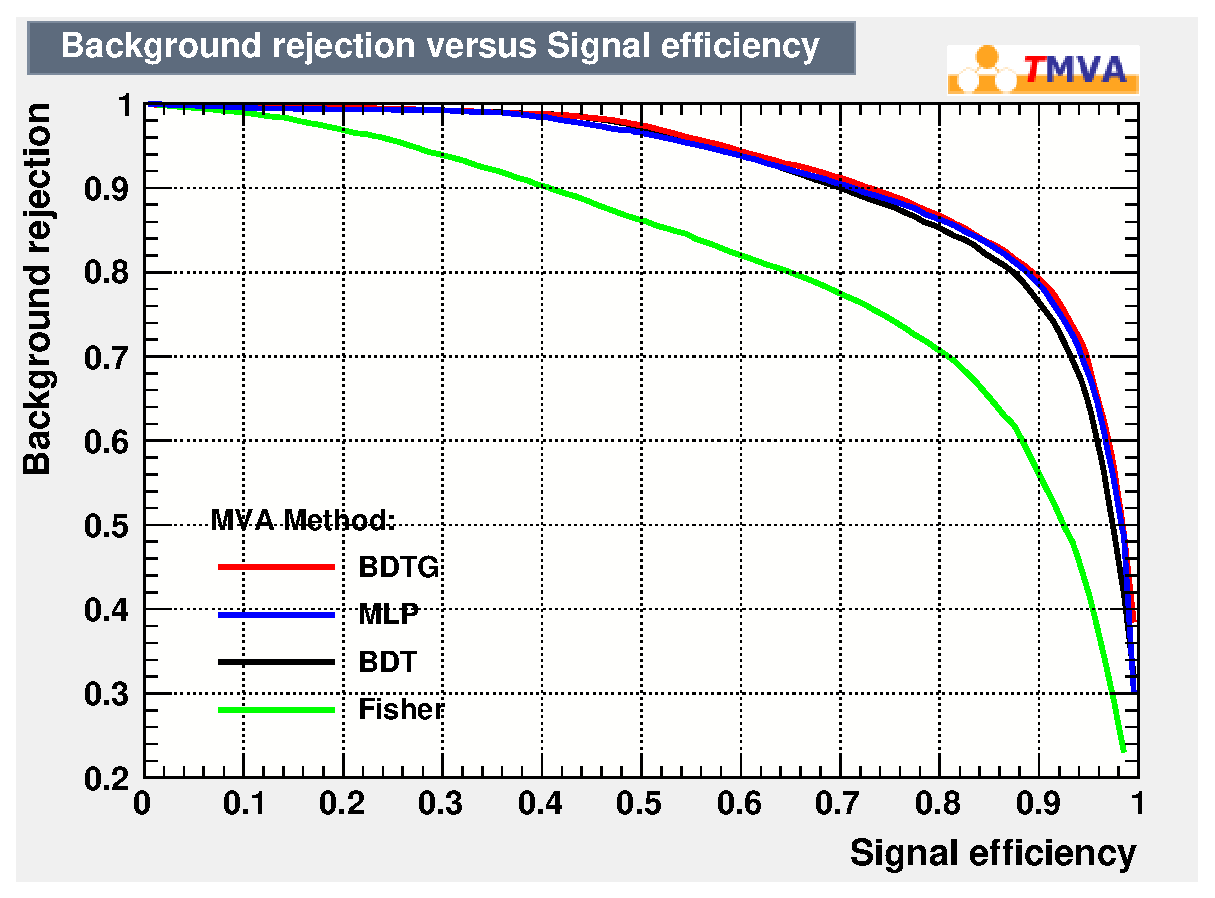
\includegraphics[width=0.49\linewidth]{Figures/06_ECAL/fast_sim/Identification/gamma_piz/no_time/rejBvsS.eps}
    \vspace*{-0.5cm}
  \end{center}
  \caption{
   Performance of different methods used on the simulation samples.
   The left one presents the performance of \g and \piz separation with the timing information included, 
   right one with the timing information excluded.
  }
  \label{fig:identi_gamma_piz_ROC}
\end{figure}
%%%%%%%%%%%%%%%%%%%%%%%%%%%%%%%%%%%%%%%%

%%%%%%%%%%%%%%%%%%%%%%%%%%%%%%%%%%%%%%%%
\begin{figure}[!htb]
  \begin{center}
    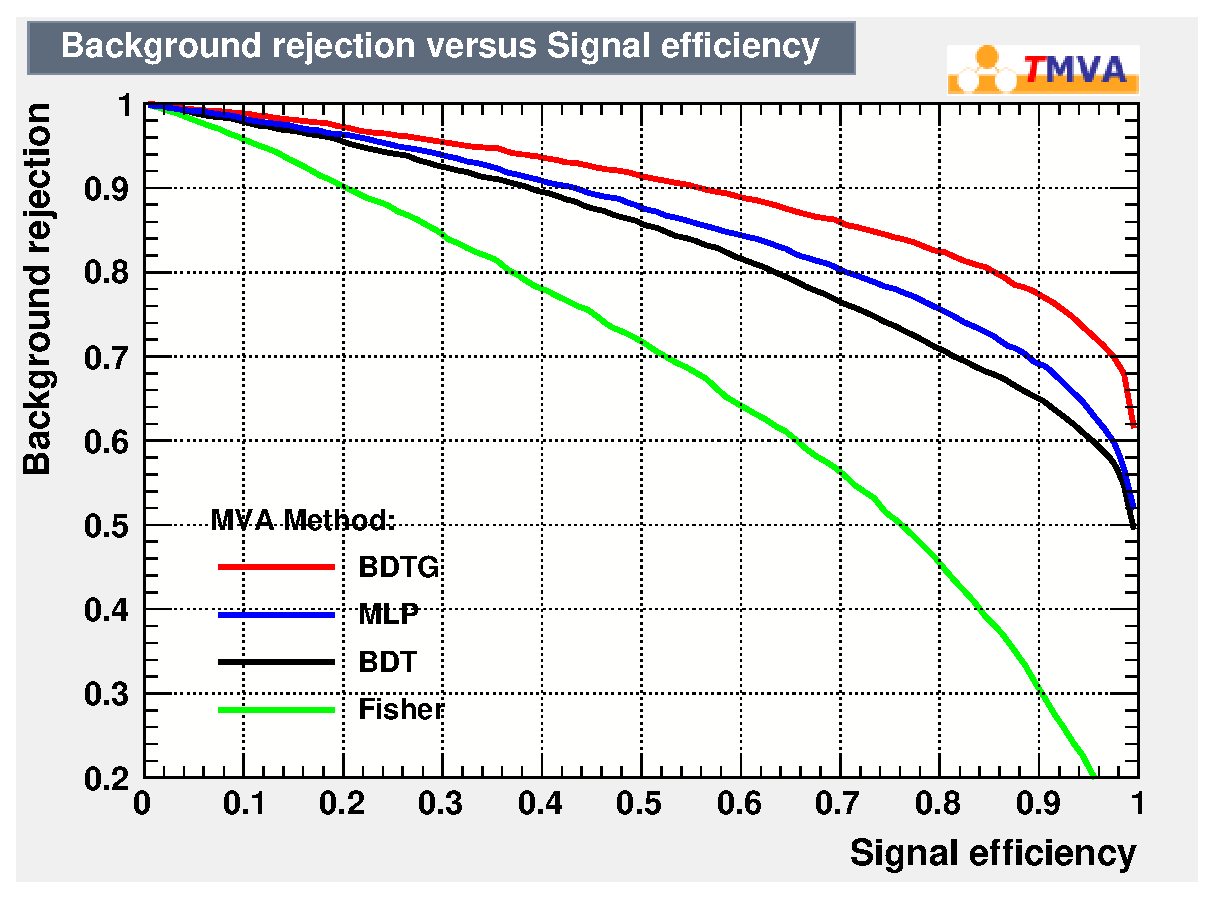
\includegraphics[width=0.49\linewidth]{Figures/06_ECAL/fast_sim/Identification/gamma_combine/with_time/rejBvsS.eps} 
    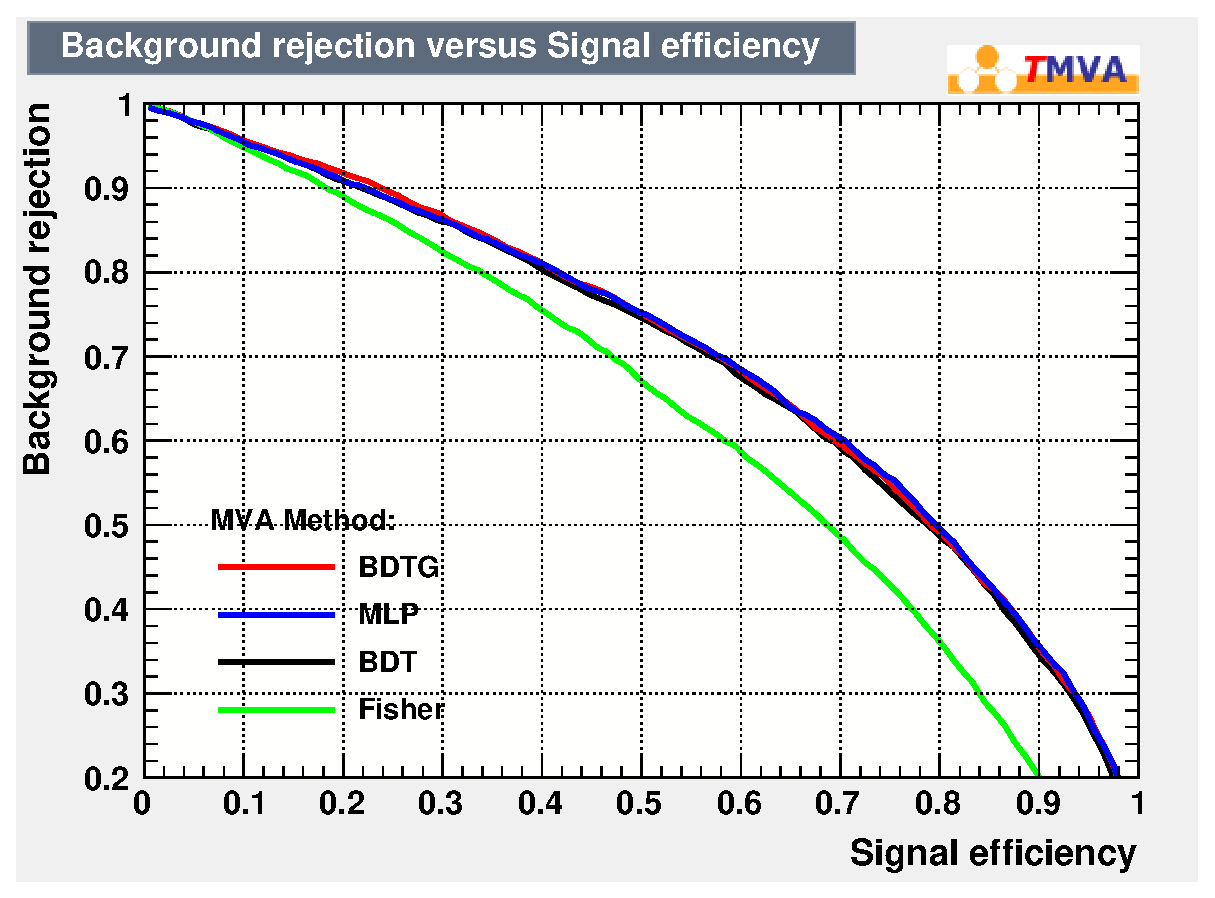
\includegraphics[width=0.49\linewidth]{Figures/06_ECAL/fast_sim/Identification/gamma_combine/no_time/rejBvsS.eps}
    \vspace*{-0.5cm}
  \end{center}
  \caption{
   Performance of different methods used on the simulation samples.
   The left one presents the performance of \g and random overlapping cluster separation with the timing information included, 
   right one with the timing information excluded.
  }
  \label{fig:identi_gamma_overlapping_ROC}
\end{figure}
%%%%%%%%%%%%%%%%%%%%%%%%%%%%%%%%%%%%%%%%

%%%%%%%%%%%%%%%%%%%%%%%%%%%%%%%%%%%%%%%%
\begin{figure}[!htb]
  \begin{center}
    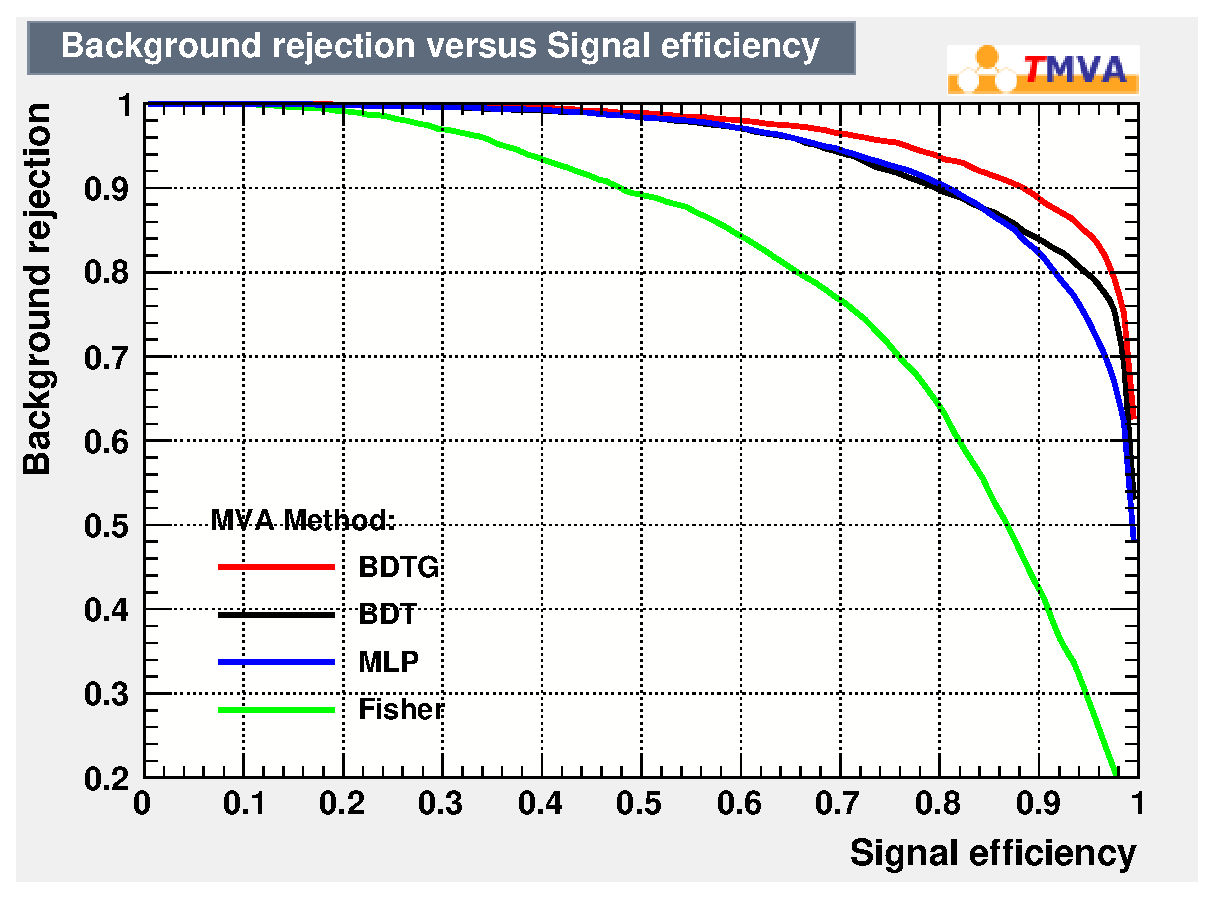
\includegraphics[width=0.49\linewidth]{Figures/06_ECAL/fast_sim/Identification/piz_combine/with_time/rejBvsS.eps} 
    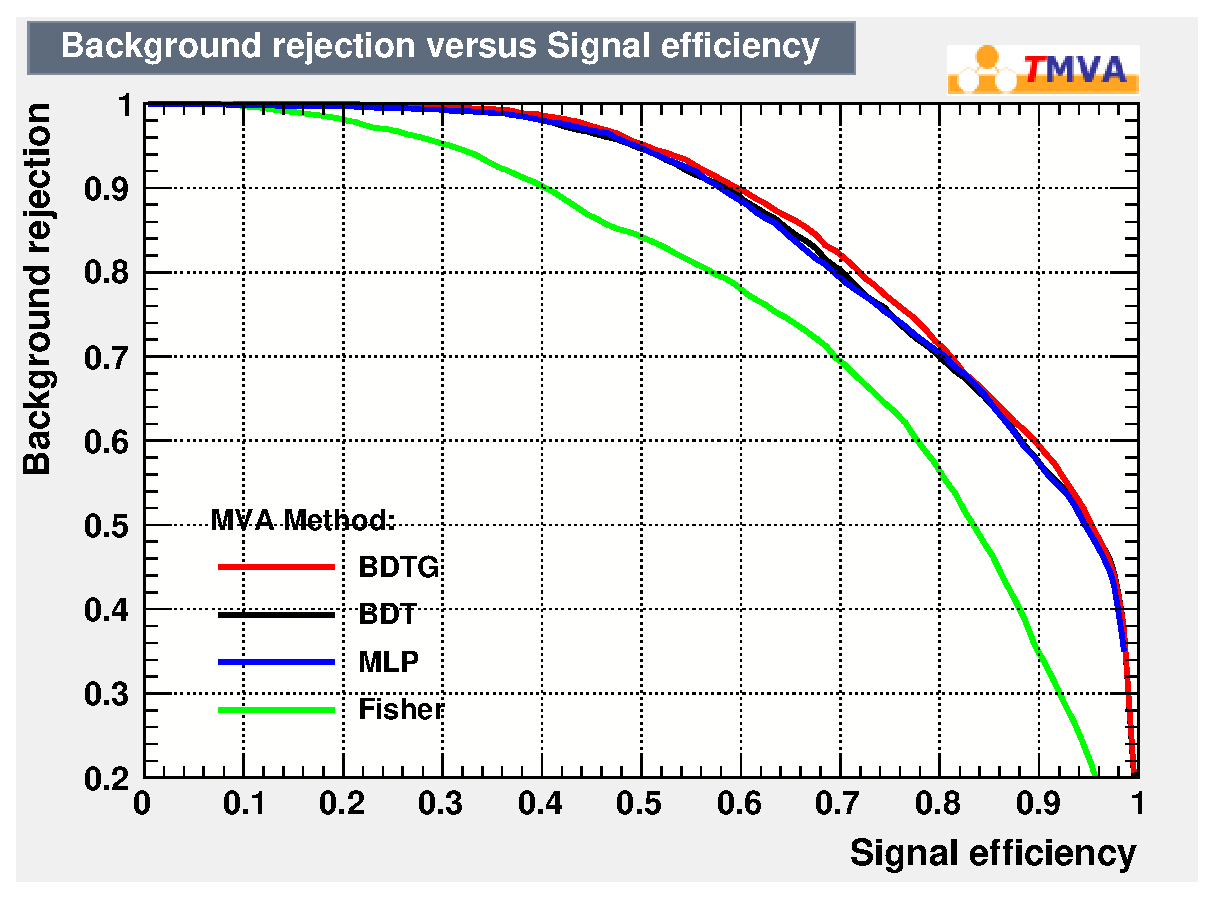
\includegraphics[width=0.49\linewidth]{Figures/06_ECAL/fast_sim/Identification/piz_combine/no_time/rejBvsS.eps}
    \vspace*{-0.5cm}
  \end{center}
  \caption{
   Performance of different methods used on the simulation samples.
   The left one presents the performance of \piz and random overlapping cluster separation with the timing information included, 
   right one with the timing information excluded.
  }
  \label{fig:identi_piz_overlapping_ROC}
\end{figure}
%%%%%%%%%%%%%%%%%%%%%%%%%%%%%%%%%%%%%%%%

Another tests are performed to identify the single \g and merged \piz from random overlapping clusters.
Figure.~\ref{fig:identi_gamma_overlapping_ROC} shows the identification ability between the pure \g and contaminated one,
from this plot, 
it is found that the timing information plays a important role for this separation.
Similar check is also performed on the merged \piz and random overlapping cluster samples,
the result is shown in the Figure.~\ref{fig:identi_piz_overlapping_ROC}.
It is obvious that BDTG method has a good performance,
three different variables are constructed to identify reconstucted cluster based on BDTG,
as listed in Table.~\ref{tab:identify}


\begin{table}[!btp]
\centering
\caption{Identification variables and corresponding functions.}
\vspace{0.2cm}
\label{tab:identify}
\begin{tabular}{c | c }\hline\hline
Variables  					& function \\\hline
${\rm PID\_g\_piz}$   		& Is a pure \g rather than a merged \piz  \\
${\rm PID\_g\_conta}$    	& Is a pure \g without contamination\\
${\rm PID\_piz\_conta}$  	& Is a merged \piz without contamination\\
\hline
${\rm Dis\_charge}$   			& Is a neutral partile rather than coming from charged track \\
\hline\hline
\end{tabular}
\end{table}






